% !TEX program = xelatex
\documentclass[11pt,aspectratio=169]{beamer}

\usetheme{Berlin}
\usecolortheme{default}

\usepackage[UTF8]{ctex}
\usepackage{amsmath,amssymb,mathtools}
\usepackage{array}
\usepackage{booktabs}
\usepackage{graphicx}
\usepackage{tikz}
\usetikzlibrary{arrows.meta,positioning,shapes.geometric}
\usepackage{hyperref}

\graphicspath{{./}{../endofnuaa_project/fig/}}

\setbeamertemplate{navigation symbols}{}
\setbeamertemplate{headline}{}
\setbeamertemplate{footline}[frame number]
\setbeamerfont{frametitle}{size=\large}
\setbeamerfont{title}{size=\Large}

\title{基于分层架构的舵机测试软件设计与实现\\毕业答辩}
\author{答辩人：易博天\\指导教师：叶永强教授}
\institute{南京航空航天大学自动化学院}
\date{2026年6月}

\begin{document}

\begin{frame}
  \titlepage
\end{frame}

\begin{frame}{答辩目录}
  \centering
  \tableofcontents[hideallsubsections]
\end{frame}

\section{课题背景与目标}

\begin{frame}{课题背景与研究目标}
  \begin{itemize}
    \item 舵机测试需要覆盖串口收发、控制激励、反馈采集、指标计算和结果留档等环节。
    \item 通信、控制和算法若分散实现，测试过程不易复查，结果也不易追溯。
    \item 本课题围绕这一需求，设计并实现一套测试软件，将通信、基础控制、性能测试和结果管理统一纳入同一软件系统。
  \end{itemize}
\end{frame}

\begin{frame}{本文完成的主要工作}
  \begin{itemize}
    \item 完成需求分析，明确通信接入、测试组织、图表展示和结果管理等软件边界。
    \item 完成系统总体架构设计，将界面、协调、通信、测试核心和结果管理分层组织。
    \item 完成通信协议与基础控制模块，实现 RS422 串口链路、双协议抽象、发送队列和反馈解析。
    \item 完成通信测试、预测试、时域测试、频域测试四类功能，并接入统一结果管理流程。
    \item 完成软件工程落地与实机联调，形成从参数输入到结果保存的基本闭环。
  \end{itemize}
\end{frame}

\section{系统实现}

\begin{frame}{系统总体架构与实现思路}
  \small
  \textbf{分层实现}

  \vspace{0.3em}
  \begin{tabular}{@{}p{0.16\textwidth}p{0.74\textwidth}@{}}
    \toprule
    层次 & 主要职责 \\
    \midrule
    界面层 & 参数录入、状态查看、结果展示 \\
    桥接层 & 暴露受控接口，隔离本地资源访问 \\
    协调层 & 统一调度串口、测试核心与文件操作，组织任务启动和状态切换 \\
    通信模块 & 完成串口收发、协议解析和反馈样本更新 \\
    测试核心 & 承担通信测试、预测试、时域测试、频域测试及指标计算 \\
    结果管理 & 支持结果保存、历史加载与测试复查 \\
    \bottomrule
  \end{tabular}

  \vspace{0.5em}
  \small
  该结构把界面交互、通信处理、测试计算和结果管理分开组织，便于功能复用与后续扩展。
\end{frame}

\begin{frame}{通信协议与基础控制实现重点}
  \begin{columns}[T,onlytextwidth]
    \column{0.54\textwidth}
    \small
    \begin{itemize}
      \item 软件支持两种协议版本，差异限制在通信层内部，上层流程统一读取控制量与反馈量。
      \item 控制帧发送采用队列串行化处理，避免手动控制、自动控制和测试任务争用同一串口。
      \item 接收流程按同步字搜索、帧长判断、完整帧提取、字段解析与校验推进，同时处理半包与粘包。
      \item 解析后的数据统一表示为帧头、载荷、校验和时间戳，直接服务于测试核心和界面显示。
    \end{itemize}

    \column{0.46\textwidth}
    \footnotesize
    \begin{tabular}{@{}p{0.18\textwidth}p{0.14\textwidth}p{0.50\textwidth}@{}}
      \toprule
      协议 & 帧长 & 关键差异 \\
      \midrule
      协议一 & 12 字节 & 固定长度帧，适用于基础控制与反馈 \\
      协议二 & 18/26 字节 & 引入帧长字段和序号字段，便于连续控制跟踪 \\
      \bottomrule
    \end{tabular}

    \vspace{0.9em}
    \small
    \textbf{接收处理阶段}\\
    同步字搜索、帧长判断、完整帧提取、字段解析与校验。
  \end{columns}
\end{frame}

\begin{frame}{软件界面与功能落地}
  \begin{columns}[T,onlytextwidth]
    \column{0.75\textwidth}
    \centering
    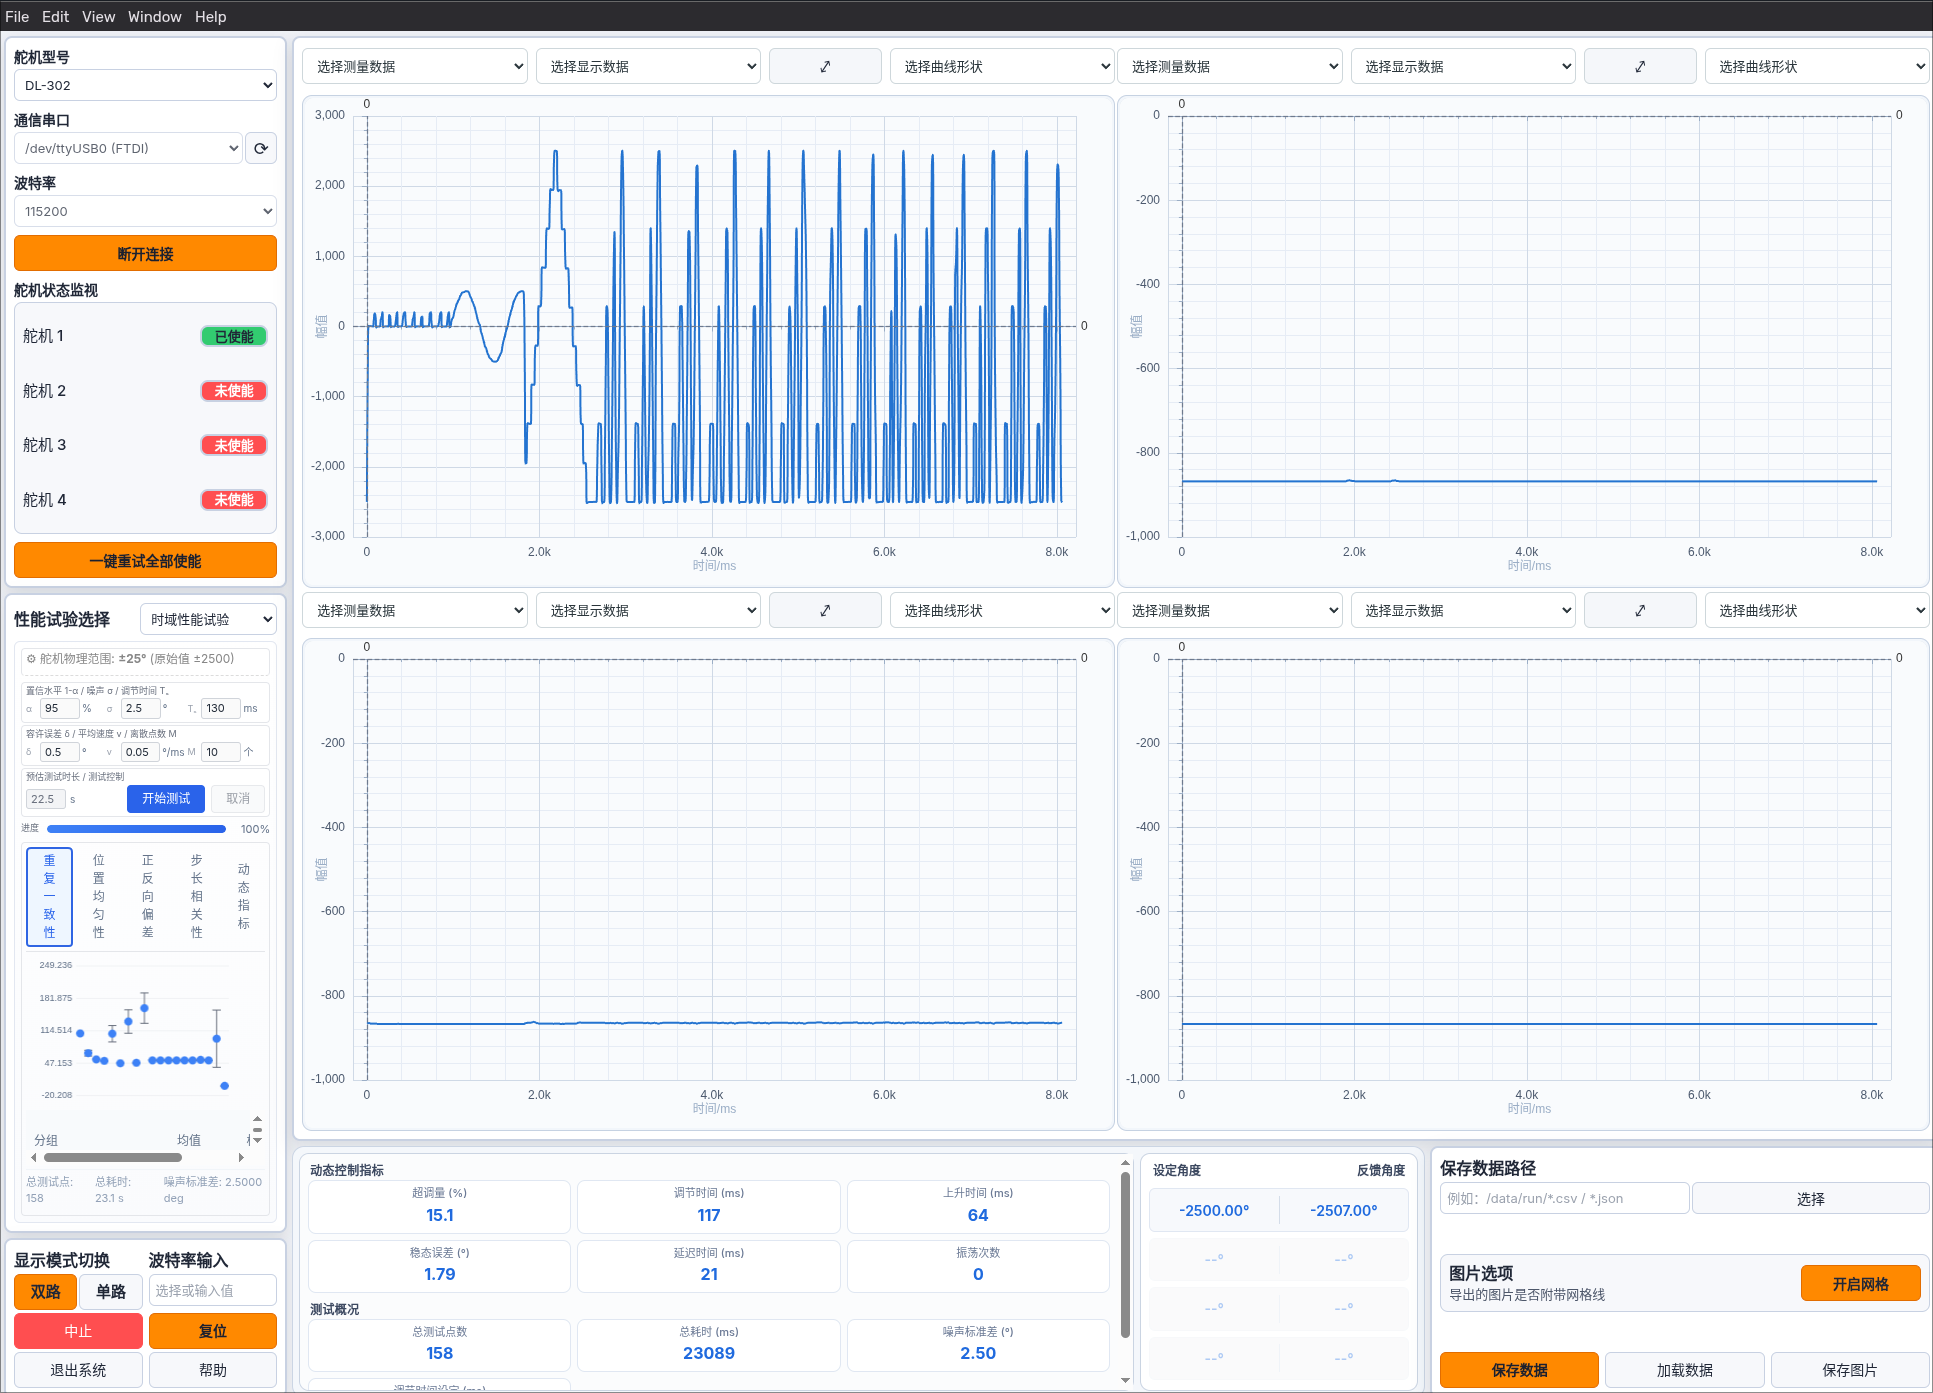
\includegraphics[width=\textwidth,height=0.72\textheight,keepaspectratio]{chapter3-layout.png}

    \column{0.35\textwidth}
    \footnotesize
    \textbf{已落地功能}
    \begin{itemize}
      \setlength{\itemsep}{0.25em}
      \item 通信选择与协议配置
      \item 测试入口与参数输入
      \item 实时曲线与状态观察
      \item 结果保存与历史加载
    \end{itemize}

    \textbf{说明}\\
    测试执行和结果复查均在此完成。
  \end{columns}
\end{frame}

\section{关键算法设计}

\begin{frame}{关键算法一：控制性能预测试}
  \begin{columns}[T,onlytextwidth]
    \column{0.40\textwidth}
    \small
    \textbf{核心设计：}
    \begin{itemize}
      \item 静止段采样：估计反馈噪声标准差。
      \item 阶跃响应测量：估计保守调节时间和平均运动速度。
      \item 参数回传：为时域和频域测试提供窗口长度、等待时间和采样规模依据。
    \end{itemize}

    \textbf{结果：}把经验参数转化为可追溯的测试输入。

    \column{0.60\textwidth}
    \centering
    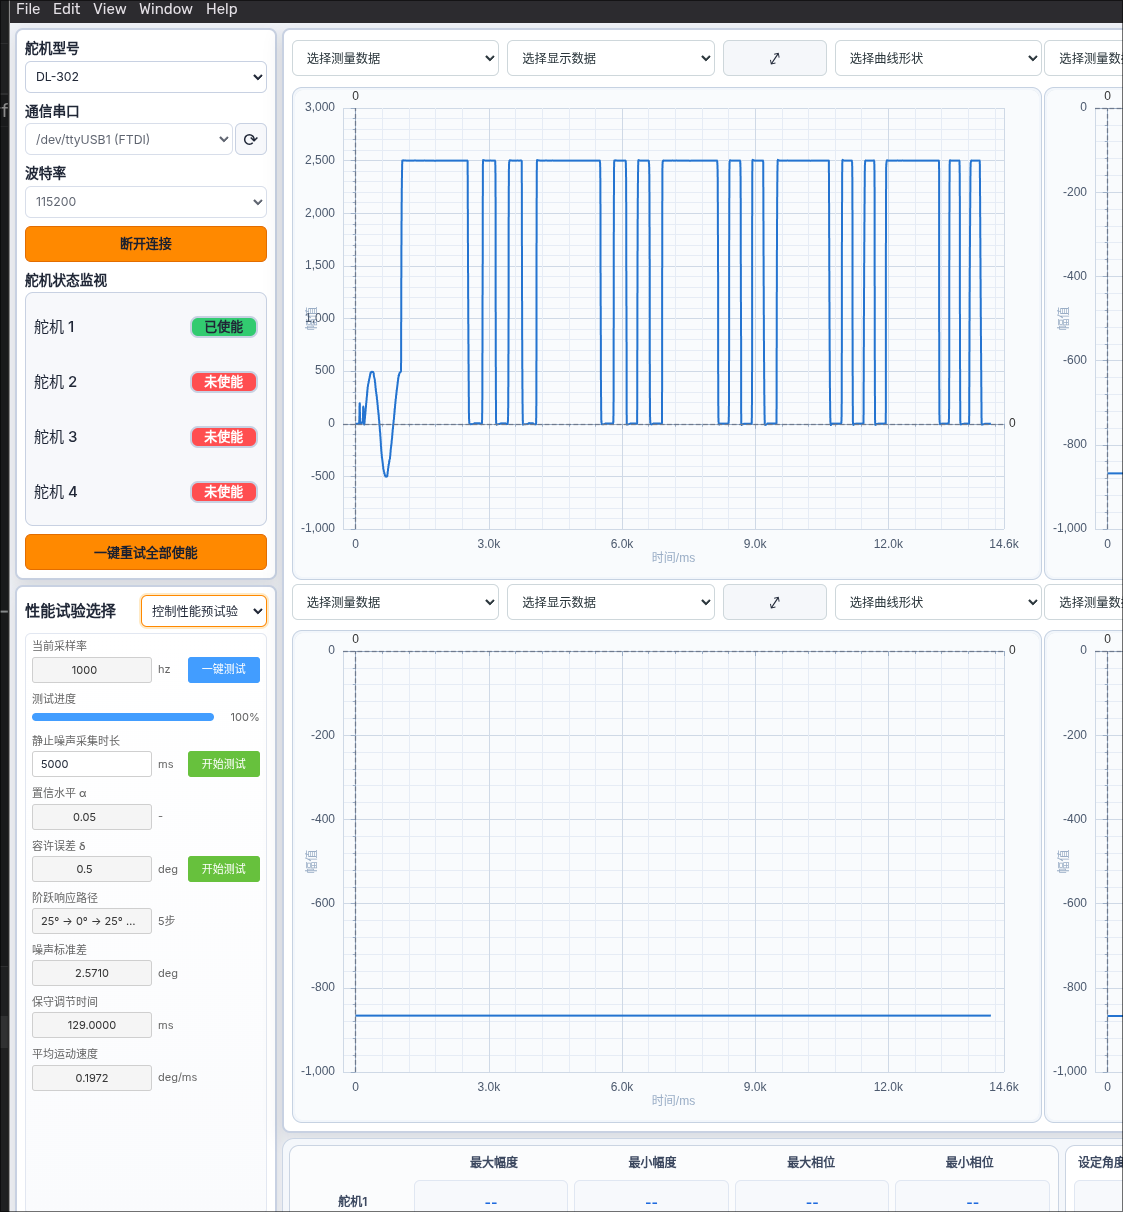
\includegraphics[width=\textwidth,height=0.68\textheight,keepaspectratio]{ch5-pretest.png}
  \end{columns}
\end{frame}

\begin{frame}{关键算法二：时域性能测试}
  \begin{columns}[T,onlytextwidth]
    \column{0.40\textwidth}
    \small
    \textbf{核心设计：}
    \begin{itemize}
      \item 在物理范围内均匀生成测试位置，组织正向、反向和重复测试路径。
      \item 根据噪声标准差、置信水平和容许误差计算统计窗口长度。
      \item 从响应曲线提取调节时间、超调量、上升时间、延迟时间、稳态误差和振荡次数。
    \end{itemize}

    \textbf{结果：}既看单点响应，也比较不同位置、方向和步长下的一致性。

    \column{0.60\textwidth}
    \centering
    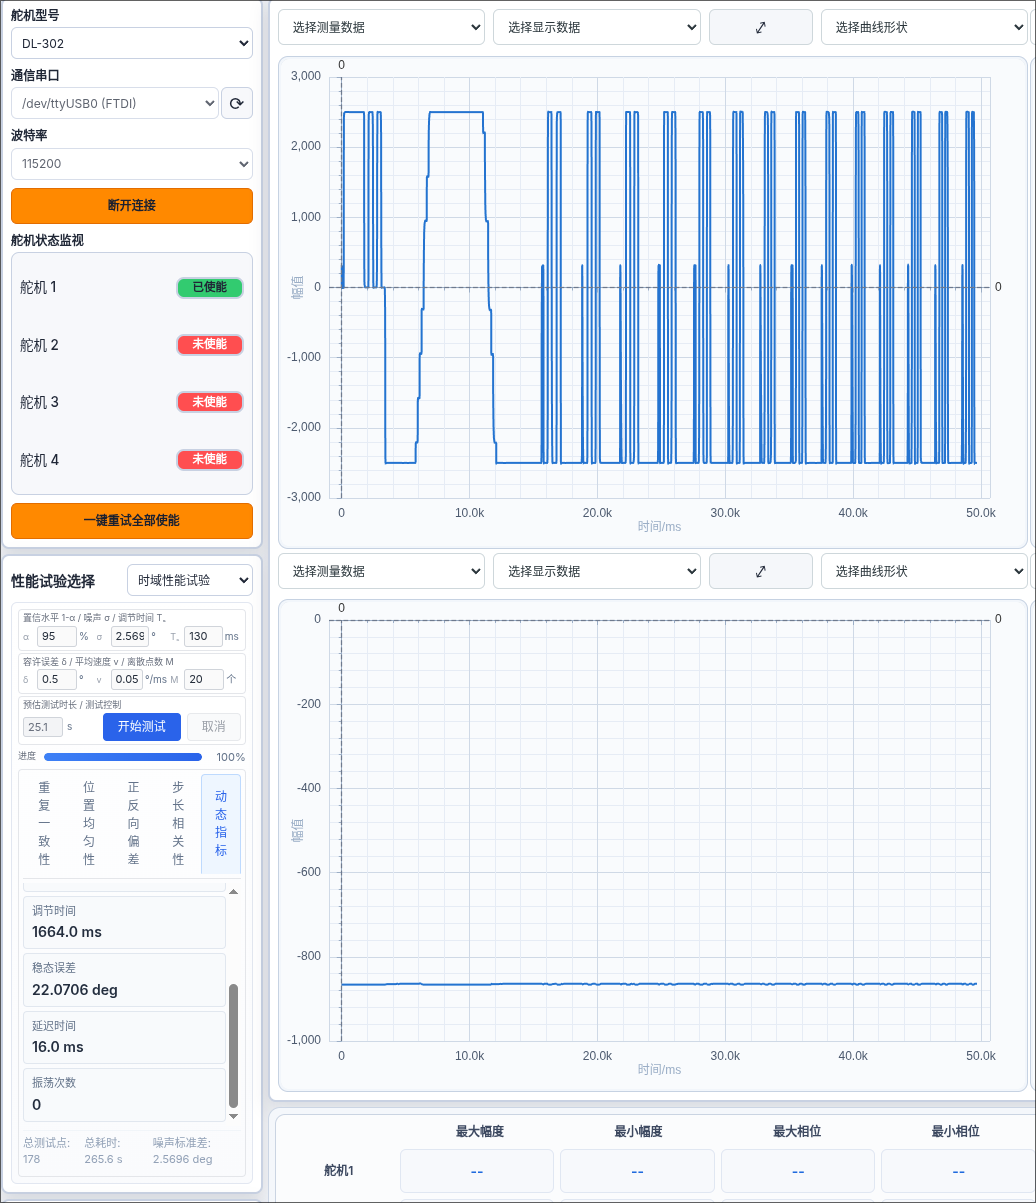
\includegraphics[width=\textwidth,height=0.68\textheight,keepaspectratio]{ch5-time-domain.png}
  \end{columns}
\end{frame}

\begin{frame}{关键算法三：频域性能测试}
  \begin{columns}[T,onlytextwidth]
    \column{0.40\textwidth}
    \small
    \textbf{核心设计：}
    \begin{itemize}
      \item 采用对数扫频生成频率点，兼顾低频分辨率与高频覆盖。
      \item 根据幅值误差、相位误差和周期覆盖要求确定每个频率点的采样规模。
      \item 采用相关法估计输出幅值与相位，形成伯德图并提取带宽、谐振频率等指标。
    \end{itemize}

    \textbf{结果：}给出与时域指标互补的频率响应评价。

    \column{0.60\textwidth}
    \centering
    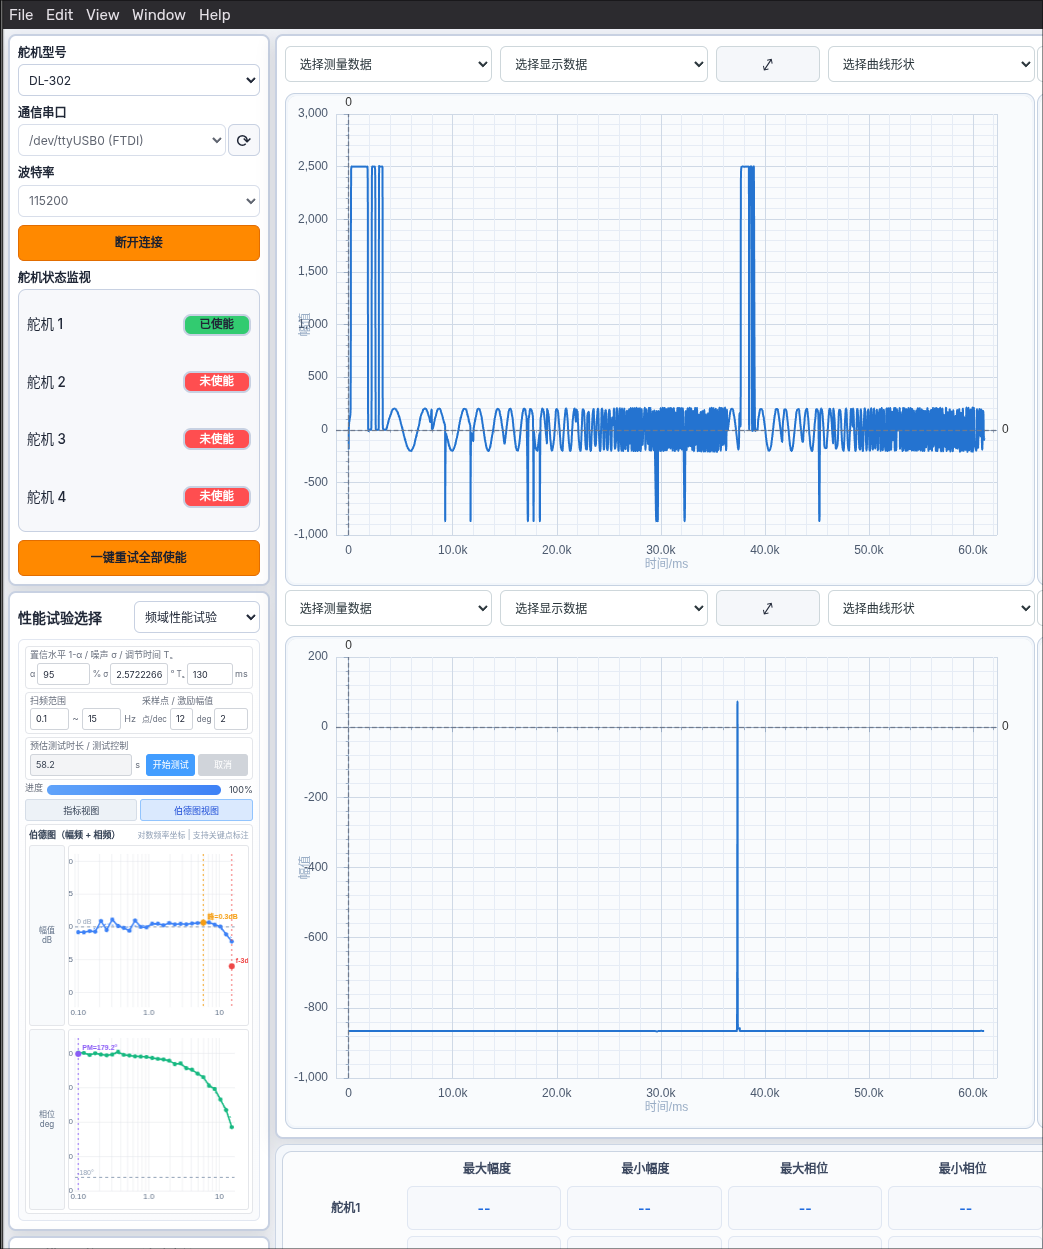
\includegraphics[width=\textwidth,height=0.68\textheight,keepaspectratio]{ch5-frequency-domain.png}
  \end{columns}
\end{frame}

\section{验证与结论}

\begin{frame}{测试验证与实现成果}
  \begin{columns}[T,onlytextwidth]
    \column{0.40\textwidth}
    \small
    \textbf{已完成验证}
    \begin{itemize}
      \item 手动链路：控制帧可持续发送，反馈帧可稳定解析。
      \item 高频自动链路：后台任务生成的控制帧能够进入真实串口发送流程。
      \item 使能检测：检测结果与当前硬件接线状态一致。
      \item 结果管理：结构化测试结果可以保存、加载并重新展示。
    \end{itemize}

    \textbf{结论}\\
    当前软件已经形成从参数输入、控制发送、反馈解析、指标计算到结果留档的基本闭环。

    \column{0.60\textwidth}
    \centering
    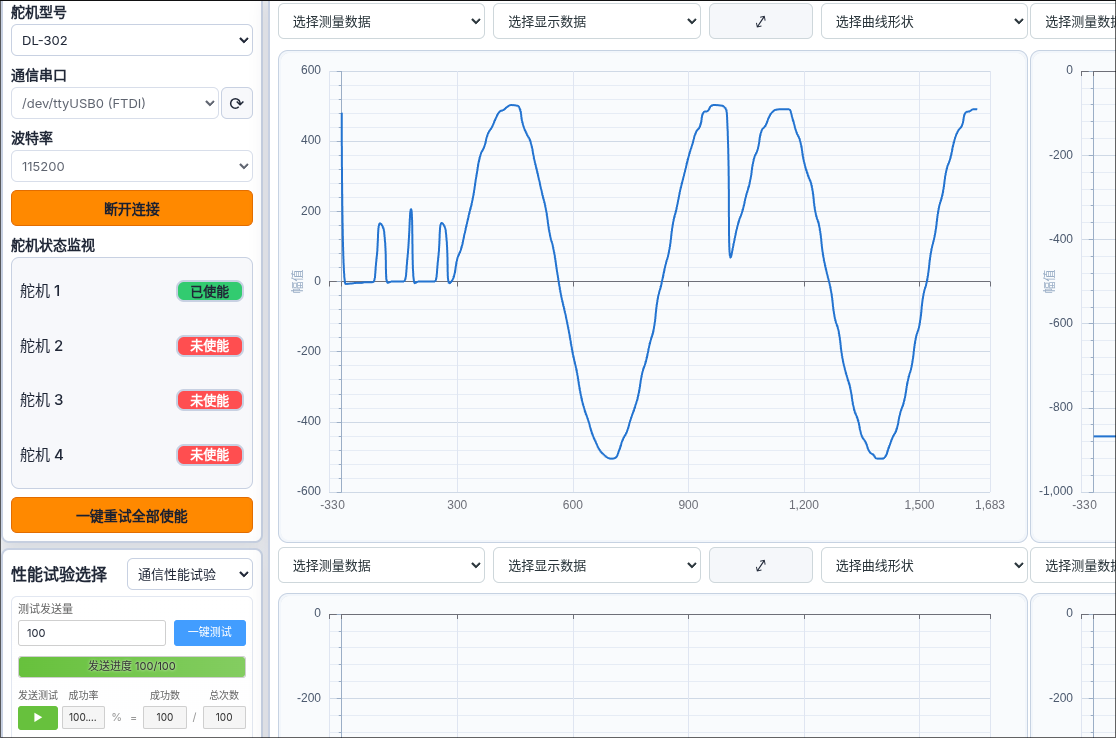
\includegraphics[width=\textwidth,height=0.70\textheight,keepaspectratio]{ch5-comm-test.png}
  \end{columns}
\end{frame}

\begin{frame}{总结与展望}
  \begin{columns}[T,onlytextwidth]
    \column{0.53\textwidth}
    \textbf{工作总结}
    \begin{itemize}
      \item 完成需求分析、分层架构设计、通信协议处理和四类测试功能实现。
      \item 将通信、基础控制、测试算法和结果管理组织到同一程序中，形成可运行、可展示、可保存的工程闭环。
      \item 通过当前实机联调验证了基础收发、自动控制链路、使能检测和结果管理等关键能力。
    \end{itemize}

    \column{0.47\textwidth}
    \textbf{后续工作}
    \begin{itemize}
      \item 补充长期稳定性、端到端时延和图片导出等专项验证。
      \item 完善更多工况下的参数敏感性分析和频域/时域结果对比分析。
    \end{itemize}
  \end{columns}
\end{frame}

\begin{frame}{答辩结束}
  \begin{center}
    \Large 谢谢各位老师\\[0.8em]
    \large 欢迎批评指正
  \end{center}
\end{frame}

\end{document}
